% =====================================================================
%  ch01c.tex ------ 第 1 章 §1.4 共形块空间与融合规则
%  原书 p.25--p.33（PDF 45--53）
% =====================================================================

% [原文 p.25]
% --- 以下为 p.25 上半 §1.3 收尾正文（命题 1.11 的证明收尾已在 ch01b 内跨块补完，此处不重复）；按 Lead 裁决补入本 chunk ---
Wess--Zumino--Witten 模型本来的目的，是对无边界的紧 Riemann 面 $\tilde\Sigma$，就所有的光滑映射 $f\colon\tilde\Sigma\to G_{\C}$ 取 $\exp(-S_{\tilde\Sigma}(f))$ 的平均，从而得到 Riemann 面 $\tilde\Sigma$ 的不变量。形式上，这由 Feynman 路径积分
\[
  \int_{f\colon\tilde\Sigma\to G_{\C}}\exp\bigl(-S_{\tilde\Sigma}(f)\bigr)\,\mathcal{D}f
\]
表示；但这样的无限维空间上的积分，在数学上还不是已确立的概念。当 $\Sigma$ 是边界同胚于 $S^{1}$ 的 Riemann 面时，固定环路群 $LG_{\C}$ 的元素 $\gamma$，在所有满足 $f\colon\Sigma\to G_{\C}$、且在边界上限制为 $\gamma$ 的映射 $f$ 上执行上述路径积分，便可期望由此定义出复线丛 $\mathcal{L}$ 的截面。这里的目标是：利用路径积分所暗示的性质，严格地构造这样的截面。已知复线丛 $\mathcal{L}$ 的截面空间上，仿射 Lie 代数 $\hat{\fg}$ 从左右两侧作用，并且含有 level $k$ 的最高权模
\[
  \bigoplus_{0\le\lambda\le k}\mathcal{H}_{\lambda}\otimes\mathcal{H}_{\lambda}^{*} .
\]
着眼于左模，则由命题 1.11 可期望：所得的截面在全纯映射 $h\colon\Sigma\to G_{\C}$ 的作用下不变。

把注意力放在 $\mathcal{H}_{\lambda}$ 中在全纯映射 $h\colon\Sigma\to G_{\C}$ 的作用下不变的元素全体上。这基本上就是下一节要构造的共形块空间。
% --- 跨块补完结束 ---

\section{共形块空间与融合规则}

\takeaway{共形块空间 $\mathcal{H}(\bm p,\bm\lambda)=\Hom_{\fg(\bm p)}(\bigotimes_j\mathcal{H}_{\lambda_j},\C)$ 是有限维复向量空间，可单射地嵌入不变张量空间。其维数由 level $k$ 的 Clebsch--Gordan 条件决定，这一规则称为融合规则；共形块的基可用三价图描述。}

Riemann 球面 $\CP^1$ 的齐次坐标记为 $[\zeta_0:\zeta_1]$，用 $z=\zeta_0/\zeta_1$ 表示从 $\CP^1$ 中去掉无穷远点 $\infty$ 所得复平面 $\C$ 上的坐标函数。

% [原文 p.26]
在 $\CP^1$ 上取 $n$ 个互不相同的点 $p_1,\dots,p_n$，把它们的坐标 $z(p_j)$（$1\le j\le n$）记作 $z_j$。当 $p_j$ 不是无穷远点时，令 $t_j=z-z_j$；当 $p_j$ 是无穷远点时，令 $t_j=1/z$。$t_j$ 给出点 $p_j$ 附近满足 $t_j(p_j)=0$ 的局部坐标。以下设 $p_j$（$1\le j\le n$）均不是无穷远点，并记 $\bm p=(p_1,\dots,p_n)$。

$\CP^1$ 上仅在 $p_1,\dots,p_n$ 处可能有极点的亚纯函数全体记作 $\mathcal{M}_{\bm p}$。令 $\fg=\mathfrak{sl}_2(\C)$，$\fg(\bm p)=\fg\otimes\mathcal{M}_{\bm p}$。按
\[
  [X\otimes f,Y\otimes g]=[X,Y]\otimes fg,\qquad X,Y\in\fg,\ f,g\in\mathcal{M}_{\bm p}
\]
定义 Lie 括号，$\fg(\bm p)$ 便具有 Lie 代数结构。

对 $\fg(\bm p)$ 的元素 $f$，把它在点 $p_j$ 附近关于局部坐标 $t_j$ 作 Laurent 展开，所得结果记作 $f_{p_j}(t_j)\in\C((t_j))$。由此得到线性映射 $\tau_j\colon\fg(\bm p)\to\fg\otimes\C((t_j))$。再把 $\fg\otimes\C((t_j))$ 到仿射 Lie 代数 $\hat{\fg}_j=\fg\otimes\C((t_j))\oplus\C c$ 的嵌入映射与 $\tau_j$ 复合，所得线性映射记作
\[
  \iota_j\colon\fg(\bm p)\longrightarrow\hat{\fg}_j .
\]
这些映射的直和给出的映射记作 $\iota\colon\fg(\bm p)\to\bigoplus_{j=1}^{n}\hat{\fg}_j$。

\begin{lemma*}{1.12}
上面定义的 $\iota\colon\fg(\bm p)\to\bigoplus_{j=1}^{n}\hat{\fg}_j$ 是单射，并且是 Lie 代数同态。
\end{lemma*}

\begin{proof}
单射性由解析延拓的唯一性立即推出。至于 $\iota$ 是 Lie 代数同态，可由命题 1.1 中描述仿射 Lie 代数中心扩张的 2-余循环的形式，以及 $\CP^1$ 上亚纯一次微分形式的留数之和为 $0$ 这一事实推出。
\end{proof}

% [Tutor Note: 这里 $\fg(\bm p)$ 的元素取值为亚纯函数，故它在 $p_i$ 处只有有限阶极点；$\iota$ 把同一个 $f$ 在各点 $p_j$ 处分别展开、再直和起来。当 $f$ 无极点时，各 $\iota_j(f)$ 只有非负次项；若对每个 $j$ 都有 $\iota_j(f)=0$，则 $f$ 在各 $p_j$ 附近恒为 $0$，由解析延拓的唯一性得 $f\equiv0$，故 $\iota$ 为单射。]

固定正整数 $k$，对每个点 $p_j$（$1\le j\le n$）配以仿射 Lie 代数 $\hat{\fg}_j$ 的一个 level $k$ 最高权不可约表示 $\mathcal{H}_{\lambda_j}$。把最高权组 $(\lambda_1,\dots,\lambda_n)$ 记作 $\bm\lambda$。

% [原文 p.27]
多重线性映射
\[
  \Psi\colon\mathcal{H}_{\lambda_1}\times\cdots\times\mathcal{H}_{\lambda_n}\longrightarrow\C
\]
中，在 $\fg(\bm p)$ 的作用下不变的全体记作 $\mathcal{H}(\bm p,\bm\lambda)$，称之为共形块的空间（space of conformal blocks）。这里 $\Psi$ 关于 $\fg(\bm p)$ 的作用不变，是指对所有的 $X\otimes f\in\fg(\bm p)$ 和 $\xi_1\in\mathcal{H}_{\lambda_1},\dots,\xi_n\in\mathcal{H}_{\lambda_n}$ 都有
\[
  \sum_{j=1}^{n}\Psi(\xi_1,\dots,(X\otimes f_{p_j})\xi_j,\dots,\xi_n)=0 .
\]
上式中的 $f_{p_j}$ 是亚纯函数 $f$ 在点 $p_j$ 附近关于 $t_j$ 的 Laurent 级数，它作用在 $\xi_j$ 上由引理 1.12 的嵌入映射 $\iota$ 定义。共形块空间的定义还可以改述如下。Lie 代数 $\fg(\bm p)$ 经由 $\iota$ 作用在张量积 $\mathcal{H}_{\lambda_1}\otimes\cdots\otimes\mathcal{H}_{\lambda_n}$ 上：
\[
  (X\otimes f)(\xi_1\otimes\cdots\otimes\xi_n)
  =\sum_{j=1}^{n}\xi_1\otimes\cdots\otimes\bigl((X\otimes f_{p_j})\xi_j\bigr)\otimes\cdots\otimes\xi_n .
\]
这样一来，把 $\mathcal{H}_{\lambda_1}\otimes\cdots\otimes\mathcal{H}_{\lambda_n}$ 看作 Lie 代数 $\fg(\bm p)$ 的表示空间，共形块的空间便可表为
\[
  \mathcal{H}(\bm p,\bm\lambda)
  =\Hom_{\fg(\bm p)}\left(\bigotimes_{j=1}^{n}\mathcal{H}_{\lambda_j},\C\right).
\]
这里把 $\C$ 看作平凡的 $\fg(\bm p)$-模，即所有 $\fg(\bm p)$ 的元素都以 $0$ 作用的表示空间。

考虑 $\CP^1$ 上的亚纯函数
\[
  f(z)=(z-z_i)^{r},\qquad r<0 .
\]
$f$ 仅在 $p_i$ 处有极点，用坐标函数 $t_i$ 表示即有 $f=t_i^{r}$。在点 $p_j$（$j\ne i$）附近把 $f$ 作 Taylor 展开，记为
\[
  f_{p_j}(t_j)=\sum_{m=0}^{\infty}a_m^{(j)}t_j^{m} .
\]
对 Lie 代数 $\fg$ 的元素 $X$，由于共形块的元素 $\Psi$ 在 $X\otimes f$ 的作用下不变，故对 $\xi_j\in\mathcal{H}_{\lambda_j}$（$1\le j\le n$）有

% [原文 p.28]
\begin{equation}
  \Psi(\xi_1,\dots,(X\otimes t_i^{r})\xi_i,\dots,\xi_n)
  =-\sum_{j,\,j\ne i}\ \sum_{m\ge0}a_m^{(j)}
  \Psi(\xi_1,\dots,(X\otimes t_j^{m})\xi_j,\dots,\xi_n) . \tag{1.15}
\end{equation}
此式在以下的讨论中将反复使用。

% [Tutor Note: 式 (1.15) 右端只对 $j\ne i$ 求和，是因为 $X\otimes t_i^{r}$ 只在 $p_i$ 有极点，在其余 $p_j$ 处是全纯的，其 Laurent 展开成为 $m\ge0$ 的 Taylor 级数；负幂项全部集中在左端的 $p_i$ 一栏。又注意 $r<0$ 使 $f$ 确在 $p_i$ 有极点，这是“移动极点”技巧的关键。]

下面说明，共形块的空间 $\mathcal{H}(\bm p,\bm\lambda)$ 可以自然地嵌入有限维的不变张量空间。设 $V_{\lambda_j}$ 是 $\fg$ 的最高权为 $\lambda_j$ 的不可约表示。$V_{\lambda_j}$ 是有限维线性空间，可看作 $\mathcal{H}_{\lambda_j}$ 的子空间。把自然嵌入映射记作
\[
  i\colon\bigotimes_{j=1}^{n}V_{\lambda_j}\longrightarrow\bigotimes_{j=1}^{n}\mathcal{H}_{\lambda_j},
\]
并把共形块空间 $\mathcal{H}(\bm p,\bm\lambda)$ 的元素 $\Psi$ 到 $\bigotimes_{j=1}^{n}V_{\lambda_j}$ 的限制 $i^{*}\Psi=\Psi\circ i$ 记作 $\Psi_0$。此时下述结论成立。

\begin{lemma*}{1.13}
限制映射 $i^{*}$ 给出单射
\[
  i^{*}\colon\mathcal{H}(\bm p,\bm\lambda)\longrightarrow
  \Hom_{\fg}\left(\bigotimes_{j=1}^{n}V_{\lambda_j},\C\right).
\]
也就是说，共形块的元素 $\Psi\colon\mathcal{H}_{\lambda_1}\otimes\cdots\otimes\mathcal{H}_{\lambda_n}\to\C$ 由其到 $V_{\lambda_1}\otimes\cdots\otimes V_{\lambda_n}$ 的限制唯一确定。
\end{lemma*}

\begin{proof}
首先说明：对共形块空间 $\mathcal{H}(\bm p,\bm\lambda)$ 的元素 $\Psi$，$i^{*}\Psi\colon\bigotimes_{j=1}^{n}V_{\lambda_j}\to\C$ 关于 $\fg$ 的作用不变，即对 $X\in\fg$、$\xi_j\in V_{\lambda_j}$（$1\le j\le n$）有
\[
  \sum_{j=1}^{n}\Psi(\xi_1\otimes\cdots\otimes X\xi_j\otimes\cdots\otimes\xi_n)=0 .
\]
这是因为 $\Psi$ 关于 $\fg(\bm p)$ 的作用不变，特别地，取 $\CP^1$ 上恒等于 $1$ 的函数 $1_{\CP^1}$，利用 $X\otimes1_{\CP^1}$ 作用下的不变性即可直接得出。

其次证明 $i^{*}$ 的单射性。利用式 (1.11) 所得的直和分解 $\mathcal{H}_{\lambda_j}=\bigoplus_{d\ge0}\mathcal{H}_{\lambda_j,d}$，令

% [原文 p.29]
\[
  \mathcal{F}_d=\bigoplus_{d_1+\cdots+d_n\le d}
  \left(\bigotimes_{j=1}^{n}\mathcal{H}_{\lambda_j,d_j}\right).
\]
特别地，$\mathcal{F}_0=\bigotimes_{j=1}^{n}V_{\lambda_j}$。为证明单射性，对 $d$ 作归纳：设共形块的元素 $\Psi$ 在 $\mathcal{F}_0$ 上为 $0$，证明它在每个 $\mathcal{F}_d$ 上的限制也为 $0$。$\mathcal{F}_d$ 中可表为
\[
  \xi=\eta_1\otimes\cdots\otimes(X\otimes t_i^{r})\eta_i\otimes\cdots\otimes\eta_n,\qquad
  X\in\fg,\ r<0,\ \eta_1\otimes\cdots\otimes\eta_n\in\mathcal{F}_{d-1}
\]
的元素 $\xi$，只需证明 $\Psi(\xi)=0$。用式 (1.15)，这由归纳假设立即推出。以上证明了所要的结论。
\end{proof}

由上述引理可知，特别地，共形块空间 $\mathcal{H}(\bm p,\bm\lambda)$ 是有限维复线性空间。其次讨论限制映射 $i^{*}$ 的像。level $k$ 的最高权不可约表示 $\mathcal{H}_\lambda$，是 Verma 模对由零向量 $\chi$ 生成的子模取商所得的模。如 1.2 节所说明，用 $d=k-\lambda+1$ 与最高权向量 $v\in V_\lambda$，$\chi$ 可表为 $\chi=(E\otimes t^{-1})^{d}v$。存在这样的零向量，说明对 $\Psi\in\mathcal{H}(\bm p,\bm\lambda)$，$\Psi_0\colon V_{\lambda_1}\otimes\cdots\otimes V_{\lambda_n}\to\C$ 除在 Lie 代数 $\fg$ 的作用下不变之外，还满足若干代数条件。具体地说，$\Psi_0$ 满足如下关系式。

\begin{proposition*}{1.14}
设 level $k$ 的最高权不可约表示 $\mathcal{H}_{\lambda_i}$（$1\le i\le n$）的最高权向量为 $v_i$，零向量为 $\chi_i=(E\otimes t_i^{-1})^{d_i}v_i$。对共形块 $\mathcal{H}(\bm p,\bm\lambda)$ 的元素 $\Psi$，作为多重线性映射，$\Psi_0\colon V_{\lambda_1}\times\cdots\times V_{\lambda_n}\to\C$ 满足
\begin{equation}
  \Psi_0(E^{m_1}\xi_1,\dots,E^{m_{i-1}}\xi_{i-1},v_i,E^{m_{i+1}}\xi_{i+1},\dots,E^{m_n}\xi_n)=0 .
  \tag{1.16}
\end{equation}
这里上式对 $\fg$ 的不可约表示 $V_{\lambda_j}$ 的任意元素 $\xi_j$（$j\ne i$，$1\le j\le n$），以及满足 $\sum_{j,\,j\ne i}m_j=d_i$ 的任意非负整数组 $m_j$（$j\ne i$，$1\le j\le n$）都成立。
\end{proposition*}

\begin{proof}
只需对 $i=1$ 的情形证明。由于 $\chi_1=(E\otimes t_1^{-1})^{d_1}v_1$ 是零向量，故

% [原文 p.30]
\[
  \Psi\bigl((E\otimes t_1^{-1})^{d_1}v_1,\xi_2,\dots,\xi_n\bigr)=0
\]
成立。
对此式左端反复应用式 (1.15)，再限制到 $V_{\lambda_1}\times\cdots\times V_{\lambda_n}$，得到
\[
  \sum_{m_2+\cdots+m_n=d_1}\frac{d_1!}{m_2!\cdots m_n!}
  \prod_{2\le j\le n}(z_j-z_1)^{-m_j}\,
  \Psi_0(v_1,E^{m_2}\xi_2,\dots,E^{m_n}\xi_n)=0 .
\]
再把 $z_1,\dots,z_n$ 看作变量，比较此式中 $\prod_{2\le j\le n}(z_j-z_1)^{-m_j}$ 的系数，即得所要结论。
\end{proof}

% [Tutor Note: (1.16) 中 $E$ 的幂 $m_j$ 全取非负、且总数恰为 $d_i=k-\lambda_i+1$，这正是零向量 $\chi_i$ 里 $E$ 的个数。证明时反复用 (1.15) 把 $t_1^{-1}$ 的极点逐个挪到 $p_2,\dots,p_n$，再比较 $\prod(z_j-z_1)^{-m_j}$ 的系数；这一“比较系数”之所以可行，是因为各 $z_j$ 与 $z_1$ 独立。]

到此为止的讨论，对一般的复单 Lie 代数 $\fg$ 也几乎同样可以展开。以下特别就 $\fg=\mathfrak{sl}_2(\C)$，把这里得到的代数关系式再详细考察一番。考察 $n=3$ 的情形。把共形块空间 $\mathcal{H}(\bm p,\bm\lambda)=\mathcal{H}(p_1,p_2,p_3;\lambda_1,\lambda_2,\lambda_3)$ 作为复向量空间的维数记作 $N_{\lambda_1\lambda_2\lambda_3}$。此时下述结论成立。

\begin{proposition*}{1.15}
与点 $p_1,p_2,p_3$ 对应的 level $k$ 的最高权 $\lambda_1,\lambda_2,\lambda_3$ 仅当满足条件
\[
  \lambda_1+\lambda_2+\lambda_3\in2\Z,\qquad
  |\lambda_1-\lambda_2|\le\lambda_3\le\lambda_1+\lambda_2,\qquad
  \lambda_1+\lambda_2+\lambda_3\le2k
\]
时，共形块空间 $\mathcal{H}(p_1,p_2,p_3;\lambda_1,\lambda_2,\lambda_3)$ 的维数 $N_{\lambda_1\lambda_2\lambda_3}$ 才为 $1$；其他情形下 $N_{\lambda_1\lambda_2\lambda_3}=0$。
\end{proposition*}

\begin{proof}
首先，如命题 1.4 所述，由 $\mathfrak{sl}_2(\C)$ 的表示论可知，
\[
  \Hom_{\mathfrak{sl}_2(\C)}(V_{\lambda_1}\otimes V_{\lambda_2}\otimes V_{\lambda_3},\C)\cong\C
\]
成立的充要条件是
\[
  \lambda_1+\lambda_2+\lambda_3\in2\Z,\qquad
  |\lambda_1-\lambda_2|\le\lambda_3\le\lambda_1+\lambda_2
\]
被满足，这称为 Clebsch--Gordan 条件。Clebsch--Gordan 条件不满足时，$\Hom_{\mathfrak{sl}_2(\C)}(V_{\lambda_1}\otimes V_{\lambda_2}\otimes V_{\lambda_3},\C)=0$。要使共形块空间 $\mathcal{H}(p_1,p_2,p_3;\lambda_1,\lambda_2,\lambda_3)$ 不为 $0$，除 Clebsch--Gordan 条件之外，还需要由 level $k$ 带来的约束

% [原文 p.31]
\[
  \lambda_1+\lambda_2+\lambda_3\le2k .
\]
下面证明这确实是必要的条件。与 1.2 节相同，取 $H,E,F$ 作为 $\mathfrak{sl}_2(\C)$ 的基。条件关于 $\lambda_1,\lambda_2,\lambda_3$ 对称，故利用命题 1.14 的关系式中 $i=1$ 的情形，对共形块空间 $\mathcal{H}(p_1,p_2,p_3;\lambda_1,\lambda_2,\lambda_3)$ 的元素 $\Psi$，有
\begin{equation}
  \Psi_0(v_1,E^{m_2}\xi_2,E^{m_3}\xi_3)=0,\qquad m_2+m_3=d_1 .
  \tag{1.17}
\end{equation}
这里 $v_1$ 是 $V_{\lambda_1}$ 的最高权向量，$\xi_2,\xi_3$ 分别是 $V_{\lambda_2},V_{\lambda_3}$ 的任意元素；又 $d_1$ 用 $k$ 与 $\lambda_1$ 表为 $d_1=k-\lambda_1+1$。不妨设 $\xi_2,\xi_3$ 是 $H$ 作用的特征向量，并设相应的特征值分别为 $\alpha_2,\alpha_3$。它们满足 $-\lambda_2\le\alpha_2\le\lambda_2$、$-\lambda_3\le\alpha_3\le\lambda_3$，且可用适当的非负整数 $n_2,n_3$ 表为 $\alpha_2=-\lambda_2+2n_2$，$\alpha_3=-\lambda_3+2n_3$。此时
\[
  H(v_1\otimes E^{m_2}\xi_2\otimes E^{m_3}\xi_3)
  =\bigl(2(k+1)-(\lambda_1+\lambda_2+\lambda_3)+2(n_2+n_3)\bigr)\,
  v_1\otimes E^{m_2}\xi_2\otimes E^{m_3}\xi_3
\]
成立。因此，只要 $2(k+1)-(\lambda_1+\lambda_2+\lambda_3)+2(n_2+n_3)\ne0$，由 $\Psi_0$ 关于 $\mathfrak{sl}_2(\C)$ 的作用不变便知 (1.17) 自动满足。若 $\lambda_1+\lambda_2+\lambda_3\le2k$，上述不等式（即 $2(k+1)-(\lambda_1+\lambda_2+\lambda_3)+2(n_2+n_3)\ne0$）恒成立，此时 Clebsch--Gordan 条件就是 $N_{\lambda_1\lambda_2\lambda_3}\ne0$ 的充要条件。又，当 $\lambda_1+\lambda_2+\lambda_3>2k$ 时，条件 (1.17) 给出与 $\mathfrak{sl}_2(\C)$ 作用下的不变性彼此独立的条件，可以证明 $N_{\lambda_1\lambda_2\lambda_3}=0$。以上完成了证明。
\end{proof}

% [Tutor Note: 关键计算里 $H$ 的特征值是 $2(k+1)-(\lambda_1+\lambda_2+\lambda_3)+2(n_2+n_3)$：$+2(k+1)$ 来自 $V_{\lambda_1}$ 与 $d_1$ 的搭配，即 $d_1+\lambda_1=k+1$。由 $\lambda_1+\lambda_2+\lambda_3\in2\Z$，$2(k+1)-(\lambda_1+\lambda_2+\lambda_3)$ 与 $2(n_2+n_3)$ 同奇偶，故它为零当且仅当 $\lambda_1+\lambda_2+\lambda_3\ge2k+2$。这解释了“$\le 2k$ 时自动满足、$>2k$ 时给出独立条件”的分界。]

把这里求得的 $N_{\lambda_1\lambda_2\lambda_3}\ne0$ 的条件称为 level $k$ 的 Clebsch--Gordan 条件。又，一般地，由各点对应的最高权得到共形块空间维数的规则，称为融合规则（fusion rule）。

如下所述，在无穷远点也赋予最高权的共形块空间，在下一节以后也将经常使用。在 Riemann 球面 $\CP^1$ 上取 $n+1$ 个互不相同的点 $p_1,\dots,p_n,p_{n+1}$，设 $p_{n+1}$ 是无穷远点。对 $p_1,\dots,p_{n+1}$ 分别赋予 level $k$ 的最高权 $\lambda_1,\dots,\lambda_{n+1}$，并记 $\bm p=(p_1,\dots,p_{n+1})$。

% [原文 p.32]
把共形块空间 $\mathcal{H}(\bm p;\lambda_1,\dots,\lambda_n,\lambda^{*}_{n+1})$ 定义为
\begin{equation}
  \mathcal{H}(\bm p;\lambda_1,\dots,\lambda_n,\lambda^{*}_{n+1})
  =\Hom_{\fg(\bm p)}\left(
  \Bigl(\bigotimes_{j=1}^{n}\mathcal{H}_{\lambda_j}\Bigr)\otimes\mathcal{H}^{*}_{\lambda_{n+1}},\C
  \right).
  \tag{1.18}
\end{equation}
$\fg(\bm p)$ 在
$\Hom_{\C}\bigl(\bigl(\bigotimes_{j=1}^{n}\mathcal{H}_{\lambda_j}\bigr)\otimes\mathcal{H}^{*}_{\lambda_{n+1}},\C\bigr)$
上的作用，与前面的定义相同，由各点处的 Laurent 展开给出。不过，$\mathcal{H}^{*}_{\lambda_{n+1}}$ 是 1.2 节所定义意义下的对偶模。再次使用引理 1.13 证明中的论述，这个共形块空间可以自然嵌入不变张量空间
\begin{equation}
  \Hom_{\fg}\left(
  \Bigl(\bigotimes_{j=1}^{n}V_{\lambda_j}\Bigr)\otimes V^{*}_{\lambda_{n+1}},\C
  \right).
  \tag{1.19}
\end{equation}
把共形块空间 $\mathcal{H}(\bm p;\lambda_1,\dots,\lambda_n,\lambda^{*}_{n+1})$ 作为复向量空间的维数记作 $N^{\lambda_{n+1}}_{\lambda_1\cdots\lambda_n}$。

首先，$n=1$ 时，
\[
  \Hom_{\fg}(V_{\lambda_1}\otimes V^{*}_{\lambda_2},\C)
\]
在 $\lambda_1=\lambda_2$ 时与 $\C$ 同构，其他情形为 $0$。对共形块空间的维数也可验证：$\lambda_1=\lambda_2$ 时 $N^{\lambda_2}_{\lambda_1}=1$，其他情形为 $0$。$n=2$ 时，$N^{\lambda_3}_{\lambda_1\lambda_2}=1$ 的充要条件是 level $k$ 的 Clebsch--Gordan 条件；不满足时 $N^{\lambda_3}_{\lambda_1\lambda_2}=0$。若在一般的复单 Lie 代数中作同样的表述，把对偶表示对应的最高权记以 $*$，则有 $N^{\lambda_3}_{\lambda_1\lambda_2}=N_{\lambda_1\lambda_2\lambda^{*}_3}$；但对 $\fg=\mathfrak{sl}_2(\C)$，任意有限维不可约表示都与其对偶表示同构，请注意此时成立 $N^{\lambda_3}_{\lambda_1\lambda_2}=N_{\lambda_1\lambda_2\lambda_3}$。$n=2$ 时的共形块空间 (1.18) 可以嵌入不变张量空间
\[
  \Hom_{\fg}(V_{\lambda_1}\otimes V_{\lambda_2},V_{\lambda_3}),
\]
故可取与张量表示 $V_{\lambda_1}\otimes V_{\lambda_2}$ 的不可约分解中的投影 $p^{\lambda_1\lambda_2}_{\lambda_3}\colon V_{\lambda_1}\otimes V_{\lambda_2}\to V_{\lambda_3}$ 相对应的共形块空间的一组基。把这组基用图 1.2 左侧的图来表示。

% [Tutor Note: 两种维数记号要分清：三点情形写 $N_{\lambda_1\lambda_2\lambda_3}$（(1.18) 之前的 $\mathcal{H}(p_1,p_2,p_3;\cdot)$），而带上标的 $N^{\lambda_{n+1}}_{\lambda_1\cdots\lambda_n}$ 表示第 $n+1$ 个权来自对偶模 $V^{*}_{\lambda_{n+1}}$。$\mathfrak{sl}_2$ 的有限维不可约表示自对偶，故两种写法数值相同；换成一般单 Lie 代数时二者不可混用。]

一般地，上述共形块空间的基，可以这样表示：给每条边配上 level $k$ 的最高权，所得图形是各顶点周围恰汇聚 $3$ 条边的、可缩的图。

% [原文 p.33]
\begin{figure}[htbp]
  \centering
  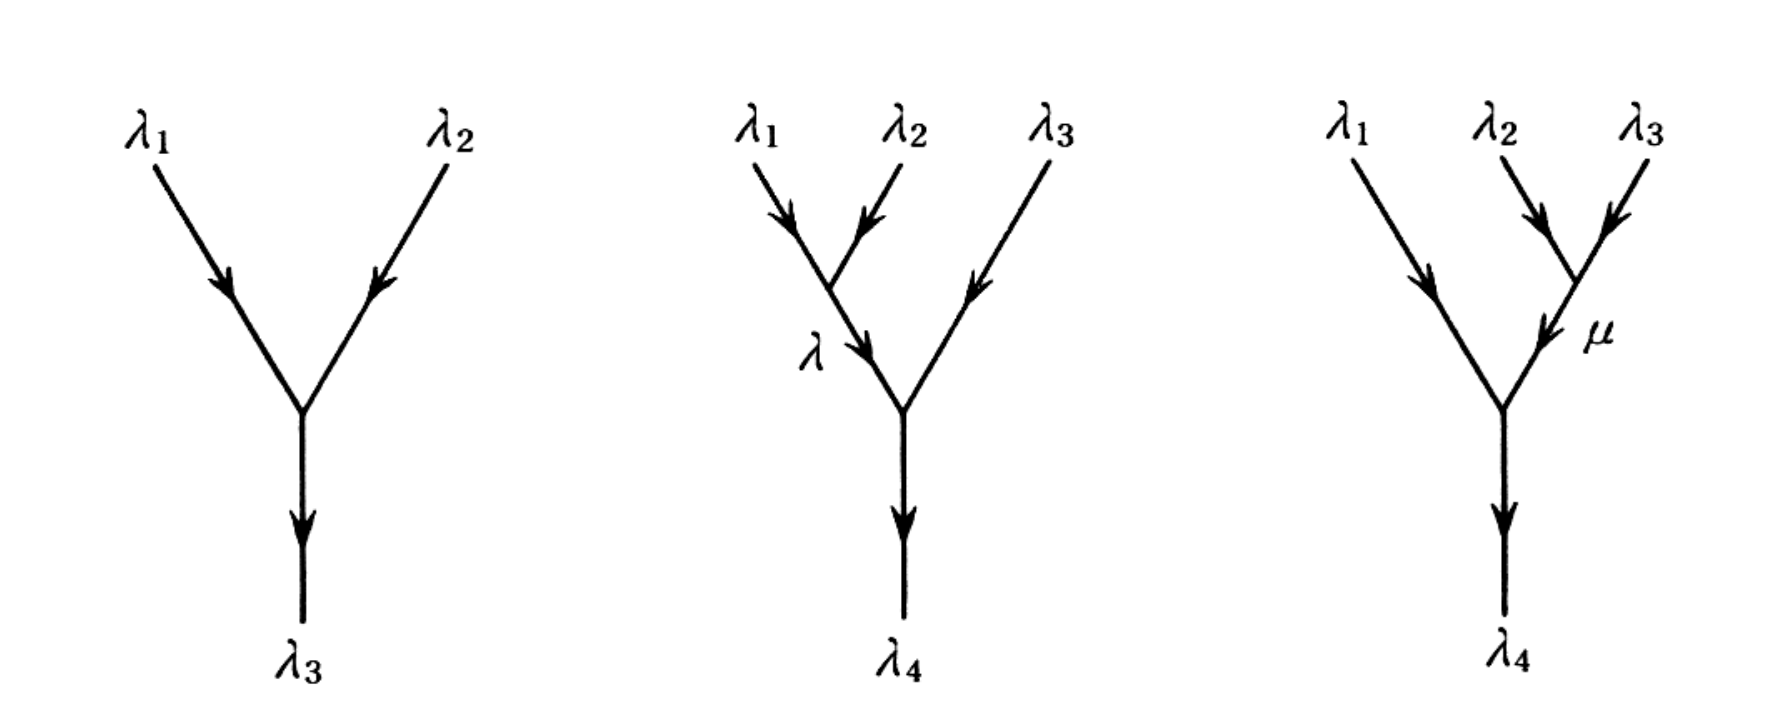
\includegraphics[width=0.88\textwidth]{figures/fig1.2.png}
  \figtitle{1.2}{左侧为 $n=2$ 的情形，中央与右侧为 $n=3$ 的情形，表示共形块空间的基（原书 p.33）}
\end{figure}

此时，外侧 $n+1$ 条边对应的最高权为 $\lambda_1,\dots,\lambda_{n+1}$，并要求汇于各顶点的 $3$ 条边所赋的最高权满足 level $k$ 的 Clebsch--Gordan 条件。图 1.2 中间的图对应射影
\[
  p^{\lambda_1\lambda_2}_{\lambda}\otimes1_{V_{\lambda_3}}\colon
  (V_{\lambda_1}\otimes V_{\lambda_2})\otimes V_{\lambda_3}
  \longrightarrow V_{\lambda}\otimes V_{\lambda_3}
\]
与
\[
  p^{\lambda\lambda_3}_{\lambda_4}\colon
  V_{\lambda}\otimes V_{\lambda_3}\longrightarrow V_{\lambda_4}
\]
的复合。利用命题 1.15 证明中的论述可知，共形块空间的基，与给图的各边赋予满足上述条件的最高权的方法一一对应。就图 1.2 中间的图而言，共形块的维数等于满足上述条件的 $\lambda$ 的个数；图 1.2 中间与右侧的图，分别对应不同的取基方式。关于这种用图描述共形块空间基的方法，下一章将再次详细讨论。

% [Tutor Note: 图中每条边上的箭头只标出该边的定向（相对顶点的指向），并不表示最高权的大小，真正约束每条边权的是三价顶点处的 level $k$ Clebsch--Gordan 条件 $\mu+\nu+\lambda\in2\Z$、$|\mu-\nu|\le\lambda\le\mu+\nu$、$\mu+\nu+\lambda\le2k$。中央与右侧两图给出同一空间的不同基，其间的变换就是下一章所说的辫子（braid）作用。]

以上讨论中，始终把 $k$ 取作正整数、用 level $k$ 的最高权表示 $\mathcal{H}_{\lambda}$ 来构造共形块空间，因而得到了源于零向量存在的代数关系式 (1.16)。若把 $k$ 取为一般值、用 Verma 模作同样的构造，则不存在这样的约束，$N_{\lambda_1\lambda_2\lambda_3}\ne0$ 的条件也变为通常的 Clebsch--Gordan 条件。

% CHUNK ch01c DONE
